
\chapter{Experimental Facility\label{ch:experiment}}

This chapter describes the experimental facility used to search for diHiggs production and other phenomena. Section~\ref{sec:CERN} covers European Organisation for Nuclear Research (CERN), the organisation
that hosts the experimental facilities. Section~\ref{sec:LHC} covers the Large Hadron Collider (LHC), the accelerator complex responsible for delivering $pp$ collisions to each experiment. Section~ref{sec:CMS}
covers the Compact Muon Solenoid (CMS), the detector which this analysis uses to study the $pp$ collisions and search for diHiggs production.


\section{CERN\label{sec:CERN}}
overview of facilities, experiments, history

\section{LHC\label{sec:LHC}}
\subsection{Overview}
The LHC is a $pp$ accelerator that straddles the border between France and Switzerland~\ref{cern-jinst-lhc}. It was installed in a 27 km tunnel with diameter 3.7 m at an average depth of 100 m underground.
The position of this tunnel with respect to nearby political and geographical points of interest is 
shown in Figrures~\ref{fig:lhc_mapwithcities} and \ref{fig:lhc_map_tuna}.
The tunnel was previously
used by the Large Electron-Positron Collider (LEP) from 1989 to 2000 for electron-positron collisions~\ref{LEP_DR1979}.

\begin{figure}[h]
 \begin{center}
    \includegraphics[width=0.90\textwidth]{figures/experiment/lhc-pho-1997-169.jpg}
      \end{center}
\caption{Map of the political and geographical highlights near the LHC~\ref{Dailler:842399}.}
\label{fig:lhc_mapwithcities}
\end{figure}

\begin{figure}[h]
 \begin{center}
    \includegraphics[width=0.90\textwidth]{figures/experiment/lhc-switzerland.pdf}
      \end{center}
\caption{Arial photo of the Geneva countryside with the LHC superimposed~\ref{Tuna:thesis}.}
\label{fig:lhc_map_tuna}
\end{figure}

The LHC is designed to accelerate protons or ions in two circular beam pipes, orbiting in opposite directions. The pre-accelerators are described in Section~\ref{sec:accelerators}, while the LHC
itself is described in Section~\ref{sec:LHC}
These beams are made to cross in four designated points of the accelerator and create collisions between
pairs of particles in opposite beams.
Each of these points is home to a large detector which measures the
products of these collisions, which are described in Section~\ref{sec:detectors}.

\subsection{Accelerator Complex\label{sec:accelerators}}

The path that a proton takes before entering a collision in the middle of CMS is shown in
Figure~\ref{fig:cern_accelerators}. Hydrogen gas is stripped of its electron and accelerated in
Linac2, a linear accelerator, to 50 MeV. Next are a series of three circular pre-accelerators that
increase the kinetic energy of the protons as well as collect the protons into discrete bunches.
These accelerators are the Proton Synchrotron Booster (PSB), the Proton Synchrotron (PS), and the
Super Proton Synchrotron (SPS), which increase the proton's energy to 1.4 GeV, 25 GeV, and 450 GeV,
respectively. 

\begin{figure}[h]
 \begin{center}
    \includegraphics[width=0.90\textwidth]{figures/experiment/lhc-pho-1991-001.jpg}
      \end{center}
\caption{The flow of the CERN accelerator complex~\ref{Jean-Luc:841493}.}
\label{fig:cern_accelerators}
\end{figure}

After the SPS, the protons are injected into the LHC, where they are accelerated to up to 7 TeV.
The bunch structure is maintained during injection into the LHC, which is important for the timing
of the collisions inside the detectors. 

\subsection{The LHC\label{sec:LHC}}

The LHC is made up of 1232 dipole magnets divided by eight insertion points. A cross sectional view
of a dipole is shown in Figure~\ref{fig:lhc_dipole}. The purpose of the
dipoles, each of which has two holes for each beam, is to direct the proton beams on their circular
path. To keep these high energy particles on their path, each dipole produces a magnetic field
of 8.3 T using a superconductor cooled with liquid helium to 1.9 K, which allows for a current
of 12 kA. The length and mass of a dipole is 14 m and 35 tons, respectively.

\begin{figure}[h]
 \begin{center}
    \includegraphics[width=0.90\textwidth]{figures/experiment/9906025_01.jpeg}
      \end{center}
\caption{Digram of a cross section of an LHC dipole~\ref{Team:40524}.}
\label{fig:lhc_dipole}
\end{figure}

Each insertion point serves a different purpose. Points 1, 2, 5, and 8 are the interaction points, where
the beams overlap to produce collisions. Point 4 contains the radio frequency cavity systems, which
provide acceleration to the particles in the direction of their motion. Points 3 and 7 contain beam
collimation systems. Point 6 contains beam dump systems for removing the beams from the LHC.

\subsection{Detectors on the LHC\label{sec:detectors}}

The general purpose detectors on the LHC are A Toroidal LHC Apparatus (ATLAS) and the Compact Muon
Solenoid (CMS), located at opposite sides of the ring at points 1 and 5, respectively. The physics
goals of these two experiements are generally the same: to search for and study the Higgs boson,
to study and improve our understanding of SM processes, and to search for BSM physics such as
SUSY or WED.

The Large Hadron Collider beauty detector (LHCb) is located at point 8 and is used
to study processes related to the bottom quark. A Large Ion Collider Experiment (ALICE) is located
at point 2 and is used to solely to study collisions when one or both beams contain lead ions. This
mode of operation of the LHC lasts about one to two months per year.

The relative positions of these four detectors on the LHC is shown in Figure~\ref{fig:lhc_detectors}.
Although the figure makes it appear that all the experiments are at the same depth, the LHC tunnel is
actually sloped at 1.5 degrees toward Lac Leman, causing the tunnel depth to vary between 50 and 150 m.

\begin{figure}[h]
 \begin{center}
    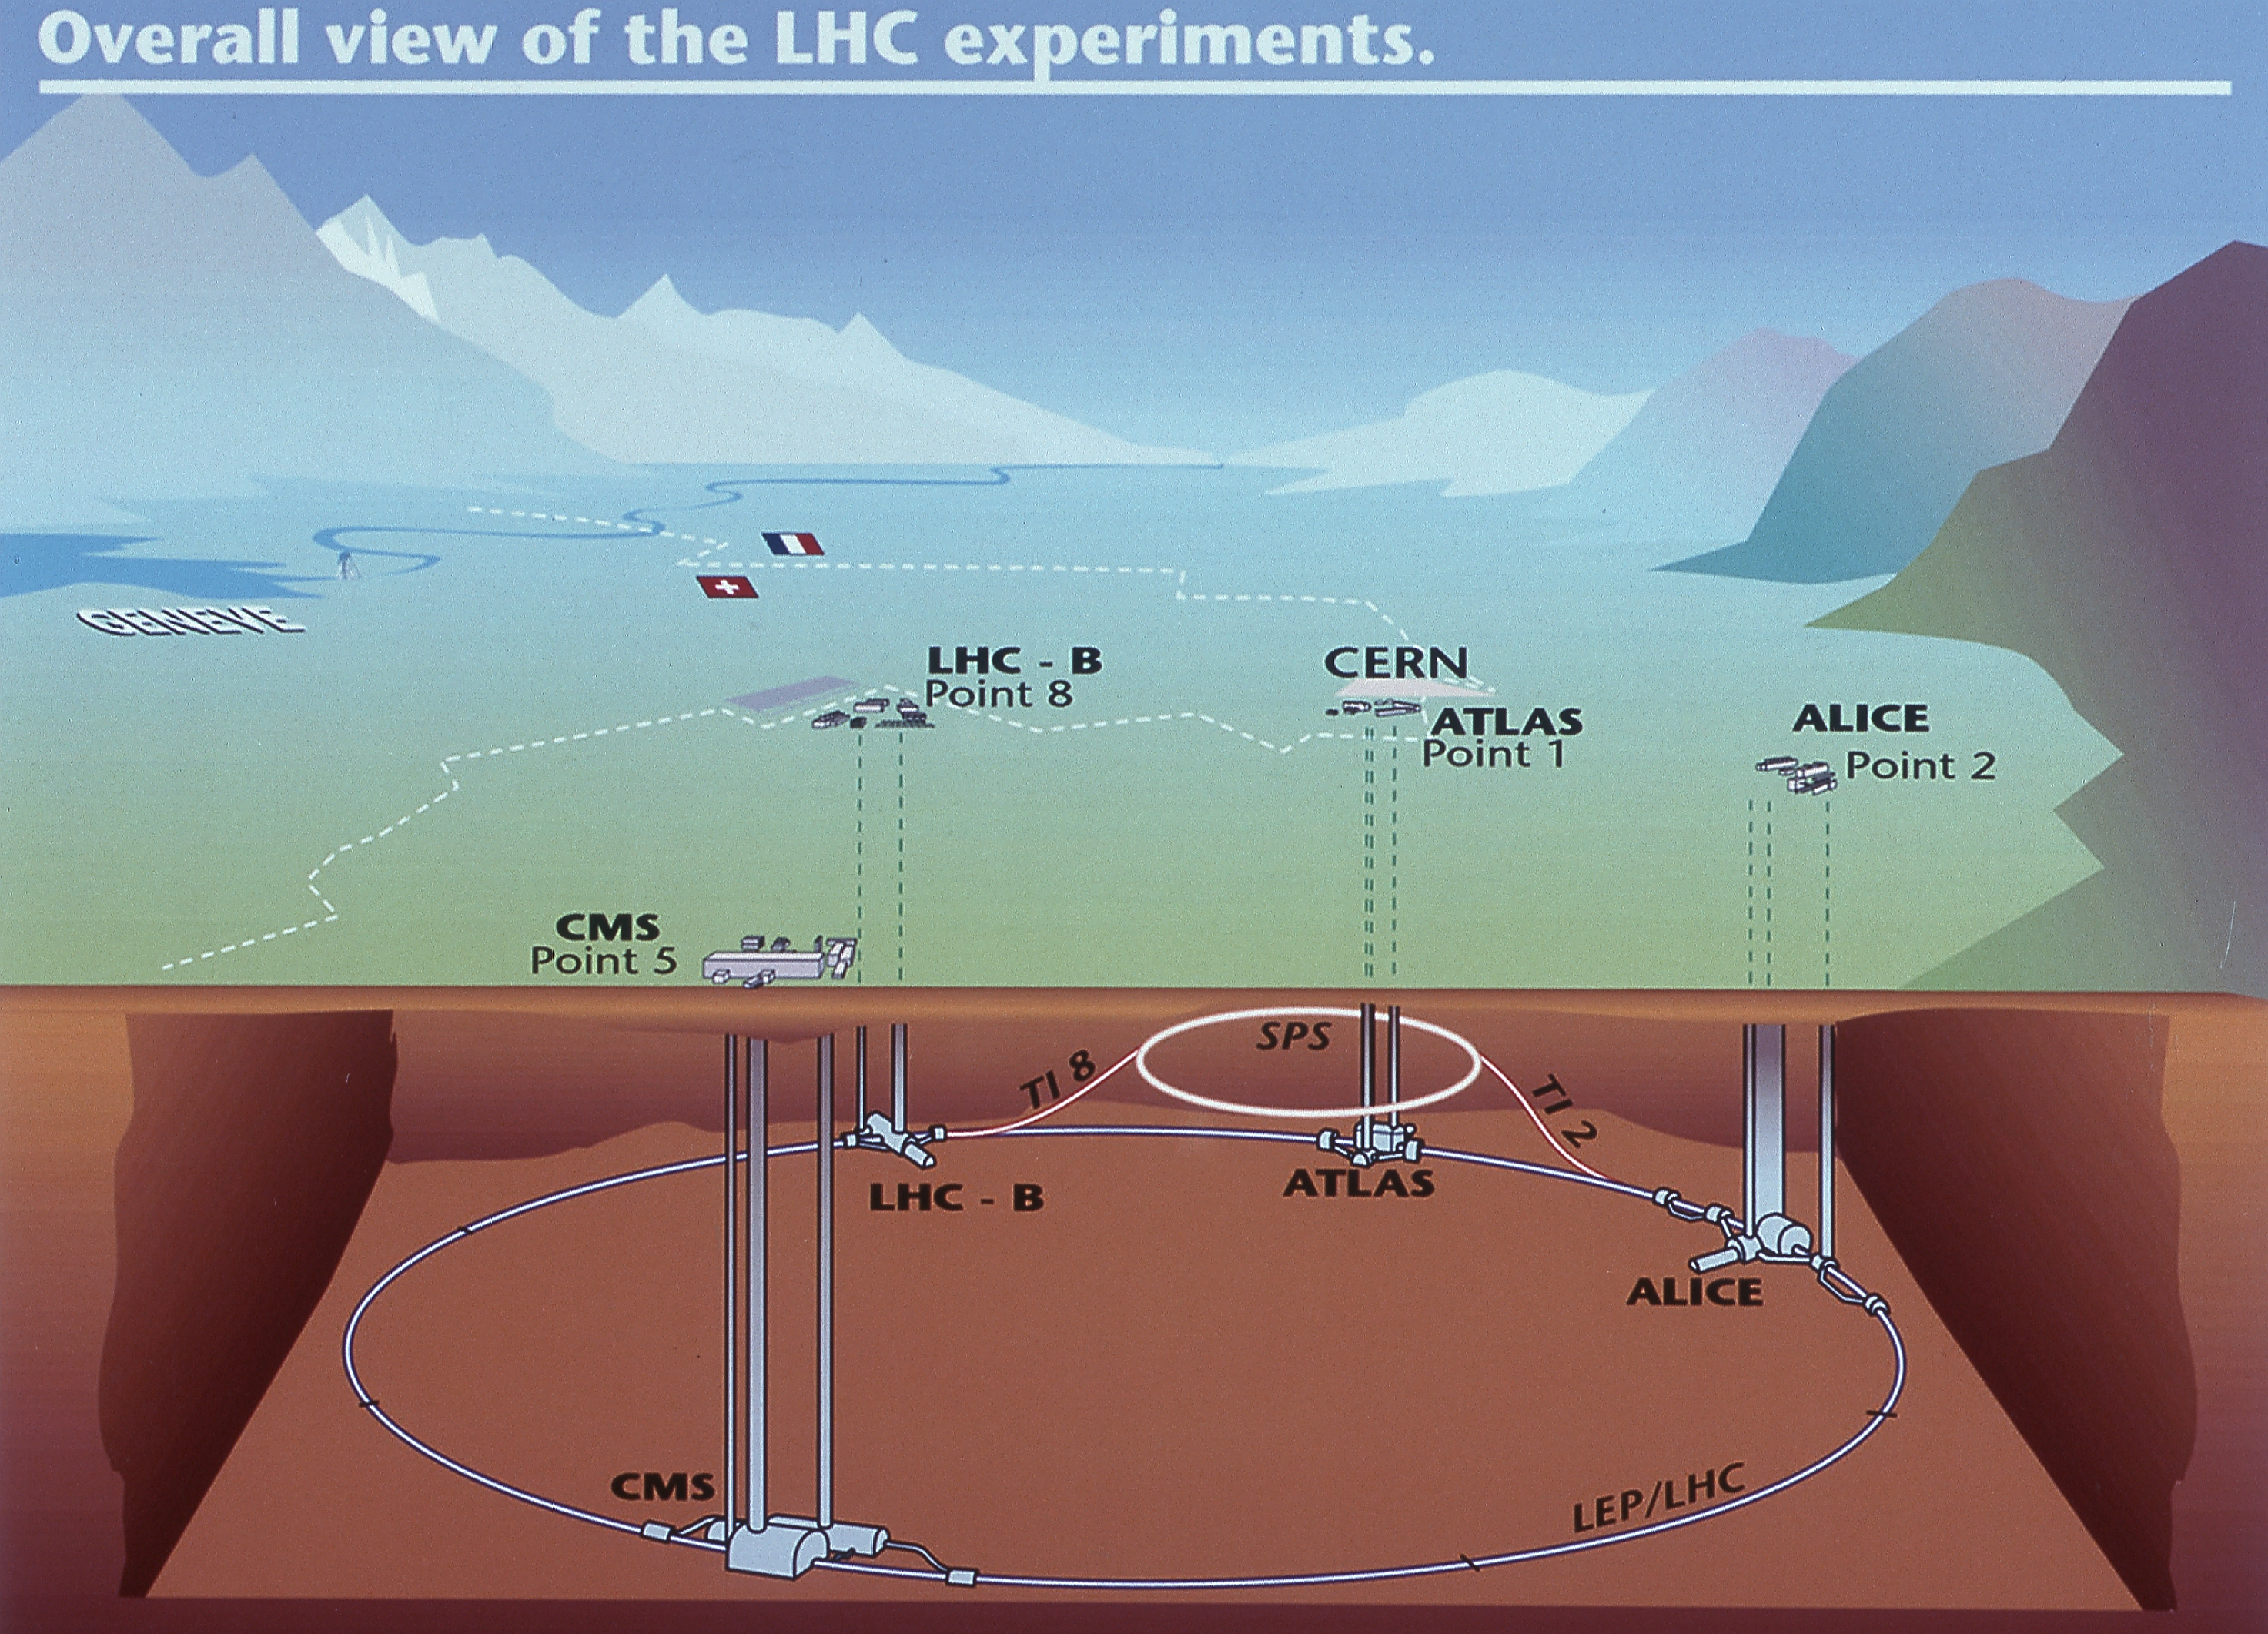
\includegraphics[width=0.90\textwidth]{figures/experiment/9906026.jpg}
      \end{center}
\caption{Underground view of the LHC and the relative positions of the four detectors~\ref{Dailler:842399}.}
\label{fig:lhc_detectors}
\end{figure}

\subsection{2012 Running}
Design parameters
The LHC is designed to deliver $pp$ collisions at a center-of-mass energy of $\sqrt{s} = 14$~TeV at a luminosity of $\mathcal{L} = \pow{10,34}$~cm$-2$s$-1$. 

\section{CMS\label{sec:CMS}}
plenty of subsections here for tracker, ecal, hcal, solenoid, muons
talk about trigger and storage later

